\scanpage{88}

Dans le cas où $\unsure{\mathscr G|G}$ est quelconque, on peut définir \unsure{cependant} le \inserted{$\unsure{L}$} $L'\unsure{:|=}\unsure{\operatorname{corad}}(L)$, qui est commutatif, et il correspond à une gerbe quotient $\unsure{\mathscr G'|G'}$ de lien commutatif $L'$. D'ailleurs, $L'$ correspond à un groupe algébrique \inserted{$H$}, et ce qui précède prouve que $(\operatorname{Ker}(\varepsilon:H\longrightarrow G_m))^{\unsure{\circ|0}}$ est un tore \uline{compact}.

\figure{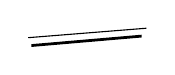
\begin{tikzpicture}\draw (0,0)--(1.5,0.12);\draw[line width=1pt] (0.04,-0.10)--(1.44,0.02);\end{tikzpicture}}

Nous envisageons maintenant une \deleted{gerbe} catégorie de motifs munie d'un \deleted{\unsure{auto}} \unsure{hom} tensoriel dans elle-même qui est ``générateur''. Ainsi $L$ est commutatif et correspond à un groupe \deleted{\unsure{commutatif}} \inserted{\unsure{alg. de type}} \deleted{$\unsure{G}$} multiplicatif $G$, \uline{muni} d'un élément $f$ (``frobenius''), et $G$ est engendré (au sens de Zariski) par $f$. \deleted{Dans le cas qui nous occupe,} \deleted{\unsure{Prenant} \illegible{3} \unsure{donné},}

\deleted{\unsure{soit}}

\mspage{87}
